\documentclass[12pt]{article}
\usepackage[utf8]{inputenc}
\usepackage[T2A]{fontenc}
\usepackage[russian]{babel}
\usepackage{amsmath}
\usepackage{amssymb}
\usepackage{dsfont}
\usepackage[dvipsnames]{xcolor}
\usepackage{setspace}
\usepackage{multirow}
\usepackage[a4paper, outer=1.5cm, inner=1.5cm, top=1cm, bottom=1cm]{geometry}
\usepackage{graphicx}
\usepackage{skull}
\usepackage{wasysym}
\usepackage{float}
\graphicspath{{.images/}}
\usepackage{hyperref}
\hypersetup{colorlinks=true, linkcolor=blue, filecolor=magenta, urlcolor=cyan}
\usepackage[firstpage]{draftwatermark}
\SetWatermarkText{
    $\qquad\qquad\qquad\qquad\qquad$\parbox{7cm}{\begin{center}
    
\includegraphics[width = 0.08\textwidth]{lion-logo.png}\bigskip\\~\bigskip\\~\vspace{-24mm}\\~\end{center}}
}
\SetWatermarkAngle{0}
\SetWatermarkScale{1.5}
\usepackage{etoolbox}

\newtoggle{ifsolved}
\newtoggle{needhelp}
\newcounter{num}
\setcounter{num}{1}

\newcommand{\newnum}{\par\textbf{\textnumero\arabic{num}}\stepcounter{num}}
\newcommand{\sol}{\vspace{3mm}\par\textbf{Решение: }}
\newcommand{\ans}{\vspace{3mm}\par\textbf{Ответ: }}
\newcommand{\hint}{\vspace{3mm}\par\textbf{Подсказка: }}
\newcommand{\mode}[1]{
\ifstrequal{#1}{0}{\togglefalse{ifsolved}\togglefalse{needhelp}}{\ifstrequal{#1}{1}{\togglefalse{ifsolved}\toggletrue{needhelp}}{\ifstrequal{#1}{2}{\toggletrue{ifsolved}\togglefalse{needhelp}}{\toggletrue{ifsolved}\toggletrue{needhelp}}}}} %if 0 - if 1 - if 2 - else
%\newenvironment{problem}[8]{%#1, #2, #3
%\parbox{\linewidth}{\vspace{4mm}\ifstrequal{#4}{(лёгкая)}{\newnum\textbf{.}}{\newnum\textbf{*.} } \\ #5}
%\iftoggle{ifsolved}{\sol #6}{}
%\iftoggle{ifsolved}{\ans #7}{}
%\iftoggle{needhelp}{\hint #8}{}}

\newenvironment{problem}[8]{%#1, #2, #3
\parbox{\linewidth}{\vspace{5mm}\ifstrequal{#4}{(лёгкая)}{\newnum\textbf{.}}{\newnum\textbf{*.} } \\ #5}
\iftoggle{ifsolved}{\sol #6}{}

\iftoggle{ifsolved}{\parbox{\linewidth}{\ans #7}}{}
\iftoggle{needhelp}{\parbox{\linewidth}{\hint #8}}{}}

\newenvironment{mylist} %custom list
{ \begin{itemize}
    \setlength{\itemsep}{0pt}
    \setlength{\parskip}{0pt}
    \setlength{\parsep}{0pt}     }
{ \end{itemize}                  }

\newenvironment{homeass}[1]{\vspace*{-1.5cm}
\iftoggle{ifsolved}{
    \section*{\center{Решение домашнего задания к #1.}}
}{
    \section*{\center{\textcolor{Sepia}{Домашнее задание к #1}}}
} \vspace{7mm}\large}

\parindent=0pt
\pagestyle{empty}
%$\!$[\arabic{class}.\arabic{num}]
%\ifnumcomp{\value{counter}}{>}{1}{true}{false}
%\definecolor{Gray}{gray}{0.9}
%\definecolor{mypink}{RGB}{219, 48, 122}
%\newcolumntype{g}{>{\columncolor{Gray}}p{2.8cm}}

\begin{document}
\large
\mode{7}
%0 for problems without hints
%1 for problems + hints
%2 for problems + solutions + answers
%else: show all

{\centering\section*{СПИСОК ЗАДАЧ}}

{\centering\subsection*{\smallskip\\\textcolor{green}{\textbf{Полезные вещи, которые можно и нужно копипастить:}}}}

\subsection*{\textcolor{Emerald}{\textbf{Полезные шпаргалки по LaTeXу:}}}

\textbf{Пример вставки рисунка:}

\begin{minipage}{\linewidth}
    \begin{minipage}{0.54\linewidth}
    см. рисунок справа\\
    Текст к собственно пикче, примерно всегда это либо развёрнутое описание, либо большая часть решения задачи --- стремимся экономить пространство, если это можно сделать.
    \end{minipage}
    \hspace{0.05\linewidth}
    \begin{minipage}{0.4\linewidth}
    \begin{figure}[H] 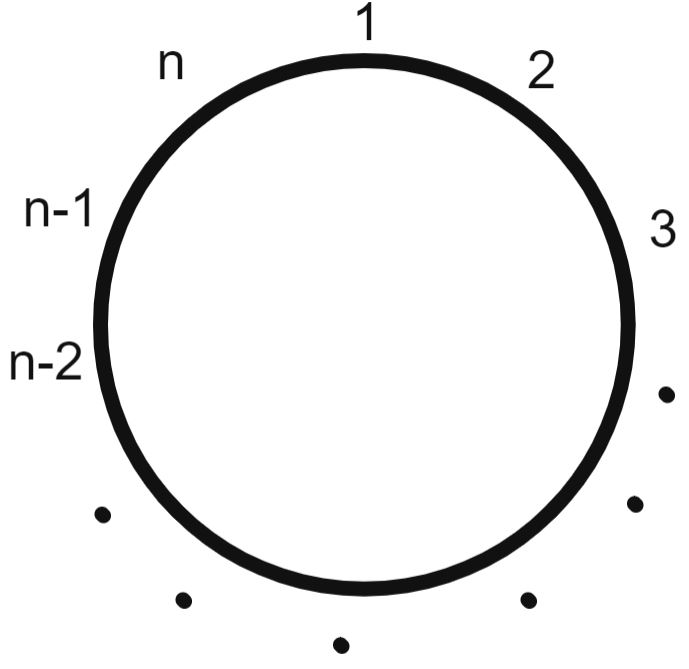
\includegraphics[width=\linewidth]{sol3} %тут поменять имя пикчи
    \end{figure}
    \end{minipage}
\end{minipage}

\textbf{Дефолтные математические знаки и символы:}\\
$\geqslant$,
$\leqslant$,
$a^{b}$,
$x_{i}$,
$\sqrt{a}$,
$\frac{a}{b}$,
$\displaystyle \frac{a}{b}$,
$\cdot$
$\;\Rightarrow\;$,
$\;\Leftrightarrow\;$,
$1{,}2$.
О промежутках:
$a\!b$,
$a\,b$,
$a\:b$,
$a\;b$,
$a\quad b$.

\textbf{Стандартные система и совокупность уравнений / неравенств:}\\
$\left\{
\begin{aligned}
f(x) &= 0 \\
g(x) &= 1
\end{aligned}\right.$

$\left[\begin{aligned}
&\left\{\begin{aligned}
f(x) &\geqslant a \\
g(x) &= b
\end{aligned}\right.\\
&\left\{\begin{aligned}
f(x) &< a \\
g(x) &= -b
\end{aligned}\right.
\end{aligned}\right.$

\subsection*{\textcolor{Emerald}{\textbf{Не математическое, но полезное:}}}
% комментарий в любом месте документа, который нигде не будет видно. Можно использовать для написания заметок-вопросов по задачам
\textbf{Пример таблицы:}

\begin{tabular}{|c|c|c|}
\hline
    $a$ & $b$ & текст
\\\hline
    $c$ & $d$ & мораль
\\\hline
\end{tabular}\\

\textbf{Отступы:} между\smallskip\\ строками\medskip\\ \textbf{Тире} --- это три дефиса.\\
\textbf{Списки:}
\begin{mylist}
\item [$\bullet$] это был пункт а
\item [2)] а это уже пункт номер 2 с изменённым заголовком
\end{mylist}

\subsection*{\textcolor{Emerald}{\textbf{Всё, неупомянутое выше (или если просто что-то не так):}}}
\begin{mylist}
\item [$\bullet$] Решение отдельных вопросов касательно ТеХа нужно искать в \href{https://www.mccme.ru/free-books/llang/newllang.pdf}{Львовском}.

\item [$\bullet$] Найти произвольный символ, который нужен, можно в \href{http://detexify.kirelabs.org/classify.html}{Detexify}.

\item [$\bullet$] Если возникли сомнения при решении, ответ практически ко всем задачам можно проверить с помощью \href{https://www.wolframalpha.com/}{WolframAlpha}.

\item [$\bullet$] Если в задаче нужно создать картинку, то лучше пока отложить эту задачу. Все графики планируется централизованно нарисовать (или перерисовать) в геогебре.

\item [\textcolor{brown}{\textbf{!!}}] Важно ставить \textcolor{red}{\textbf{$\spadesuit$}}
(или просто red) в тело задачи в случае серьёзных вопросов к решению и какой-то вопиющей лажи.

\item [\textcolor{brown}{\textbf{!!}}] Важно ставить \textcolor{olive}{\textbf{$\spadesuit$}}
(или просто olive) в тело задачи в случае не самого удачного текста и кривых отступов.
\end{mylist}

\subsection*{\textcolor{Violet}{\textbf{Комментарии:}}}% а также невидимые комментарии - так можно оставлять заметки-вопросы прямо в задаче, чтобы потом было понятно, в чём вопрос.
\begin{mylist}
\item [$\skull$] Переставлять задачи местами --- очень плохая идея.

\item [$\smiley$] При двойном клике по тексту pdf справа происходит автоматический переход к этому месту в латех-коде, а для обратного перехода можно нажать стрелку вправо (висит сверху между pdf и латех-кодом).

\item [$\smiley$] Если есть размышления, дописывать red/olive к задаче или не дописывать, то лучше всё-таки дописать.

\item [$\skull$] Самое плохое, что можно сделать --- написать в любое поле из трёх (НаписанноеРешение/ВерныйОтвет/Подсказка) только половину того, что надо, никак это не отметить, и потом пойти дальше.\\ Нужно в этот момент писать red/olive в случайном месте задачи, чтобы потом вычислить это с помощью Ctrl+F по всему документу (и это то, что потом будет делаться долго и тщательно)
\end{mylist}

\newpage
\setcounter{num}{602}

\hypertarget{7.5}{{\centering\section*{\bigskip\\\textcolor{Blue}{\hyperlink{start2}{\textcolor{Blue}{7.5}} Многочлены.}\vspace{-5mm}}}}

\begin{problem}{Понятие многочлена, его стандартный вид.}{7.5.5}{79I}{*}
{Является выражение $2x^2 - x^2 + 5$ двучленом или трёхчленом?}
{Это выражение содержит три слагаемых: $2x^2$, $-x^2$, и 5.\\ Таким образом, это трёхчлен.}
{Это трёхчлен. Двучленом это выражение может стать, только если привести его к стандартному виду: $\;\textcolor{orange}{\underline{\underline{2x^2}}} - \textcolor{orange}{\underline{\underline{x^2}}} + 5 = x^2 + 5$.}{Сколько слагаемых (членов) в этом выражении и чему они равны?}
\end{problem}

\begin{problem}{Понятие многочлена, его стандартный вид.}{7.5.5}{79I}{*}
{Может ли сумма одночленов быть одночленом?}
{Сумма любых двух одночленов является суммой двух слагаемых, то есть по определению это двучлен. Однако, после приведения к стандартному виду, если есть подобные слагаемые, это выражение может стать одночленом.}
{Может, но только после приведения многочлена к стандартному виду. Например: $3x + 4x = 7x$~--- одночлен.}{Сколько слагаемых в этом выражении?}
\end{problem}

\begin{problem}{Сложение и вычитание многочленов.}{7.5.6}{79I}{(лёгкая)}
{Найти $c$, если $\;\displaystyle \frac{a + b + c}{3} = \frac{a + b - c}{3}$.}
{Знаменатели дробей равны. Значит, равны и числители.\\ Домножим обе части уравнения на 3: получим, что $a + b + c = a + b - c$.\\
Поскольку в обеих частях уравнения есть $a$ и $b$, вычтем $a$ и $b$ из обеих частей уравнения. Получаем, что $c = -c$. Решаем это уравнение: переносим $c$ влево и делим пополам: $c = -c \;\Rightarrow\; 2c = 0 \;\Rightarrow\; c = 0$. $\,c$ найдено: оно равно нулю.}
{$c = 0$.}{Если равны две дроби с равными знаменателями, то и их числители равны.}
\end{problem}

\begin{problem}{Умножение многочленов, распределительный закон и ФСУ.}{7.5.7}{6S}{*}
{Найти все пары натуральных чисел, разность квадратов которых равна 45.}
{Пусть эти два числа --- $a$ и $b$, и $a$ --- большее число. Тогда $a^2 - b^2 = 45$. Используем формулу разности квадратов, получаем, что $(a - b)(a + b) = 45$.\\ Как можно разложить 45 на множители? $45 = 1\cdot45 = 3\cdot15 = 5\cdot9$.\\ Найдём $a$ и $b$ в каждом случае. Если $a - b = 1$, $a + b = 45$, то $a = 23$, $b = 22$.\\
Если $a - b = 3$, $a + b = 15$, то $a - b + a + b = 2a = 18$, $a = 9$, $b = 6$.\\
Если $a - b = 5$, $a + b = 9$, то $a - b + a + b = 2a = 14$, $a = 7$, $b = 2$.}
{Таких пар натуральных чисел три: 2 и 7, $\,$6 и 9, $\,$22 и 23.}{Пусть эти два числа --- некоторые неизвестные $a$ и $b$.\\ Используй формулу разности квадратов и перебери все варианты.}
\end{problem}

\begin{problem}{Умножение многочленов, распределительный закон и ФСУ.}{7.5.7}{6K}{(лёгкая)}
{После того, как длина участка выросла на $2$ м, а ширина~--- уменьшилась на $1$ м, общая площадь участка выросла на $13$ м$^2$. Как выглядит участок сейчас, если вначале его длина была на $5$ м больше ширины?}
{Пусть вначале одна сторона участка была равна $L$ м, а другая~--- $L + 5$ м (мы знаем, что вначале длина была на 5 м длиннее ширины).\\ Тогда после изменения длины и ширины длина участка будет равна $L + 5 + 2 =\\ L + 7$ м, а ширина участка будет равна $L - 1$ м. Вначале площадь участка составляет $L(L + 5)$, а после изменений~--- $(L - 1)(L + 7)$.\\ Отсюда получается уравнение: $L(L + 5) + 13 = (L - 1)(L + 7)$. Раскроем скобки: получаем, что $L^2 + 5L + 13 = L^2 - L + 7L - 7 \;\Rightarrow\; 5L + 13 = 6L - 7$. Уравнение получилось не квадратным, а линейным, решаем его: $5L + 13 = 6L - 7 \;\Rightarrow\; 20 = L$. Итого, вначале $L$, ширина участка, равна 20м, а длина равна 25 метрам.\\ Теперь же ширина участка составляет 19 метров, а длина~--- 27 метров.}
{Сейчас участок имеет вид прямоугольника с шириной 19 метров и длиной 27 метров.}{Обозначь ширину участка за $L$, составь уравнение и реши его.}
\end{problem}

\begin{problem}{Умножение многочленов, распределительный закон и ФСУ.}{7.5.7}{7A}{(лёгкая)}
{Решить уравнение: $\displaystyle\frac{(x + 2)(3x - 1)}{35} - \frac{(x + 3)(x - 2)}{14} = \frac{(x + 1)(x - 3)}{70}$.\vspace{-4mm}\\}
{Несложно подметить, что все знаменатели делятся на 7.\\ Поэтому домножим на 7 и левую, и правую части уравнения: получаем, что \vspace{-3mm}\\$$\frac{(x + 2)(3x - 1)}{5} - \frac{(x + 3)(x - 2)}{2} = \frac{(x + 1)(x - 3)}{10}.$$
$$ \text{Раскрываем скобки:} \quad\!\frac{3x^2 - x + 6x - 2}{5} - \frac{x^2 - 2x + 3x - 6}{2} = \frac{x^2 - 3x + x - 3}{10} \;\Rightarrow$$
$$ \quad\frac{3x^2 + 5x - 2}{5} - \frac{x^2 + x - 6}{2} = \frac{x^2 - 2x - 3}{10} \;\Rightarrow$$
$$ \quad\frac35 x^2 + \frac55 x - \frac25 - \left(\frac12 x^2 + \frac12 x - \frac62\right) = \frac{1}{10} x^2 - \frac{2}{10} x - \frac{3}{10} \;\Rightarrow$$
$$ \text{Раскрываем скобки:}\quad\frac35 x^2 - \frac12 x^2 - \frac{1}{10} x^2 + \frac55 x - \frac12 x + \frac{2}{10} x - \frac25 + \frac62 + \frac{3}{10} = 0 \;\Rightarrow$$
$$ \quad\frac{6 - 5 - 1}{10} x^2 + \frac{10 - 5 + 2}{10} x + \frac{-4 + 30 + 3}{10} = 0 \;\Rightarrow\; 0x^2 + \frac{7}{10} x + \frac{29}{10} = 0 \;\Rightarrow$$
$$\text{Домножим всё на 10:} \quad\frac{7}{10} x + \frac{29}{10} = 0 \;\Rightarrow\; 7x + 29 = 0 \;\Rightarrow\; 7x = -29 \;\Rightarrow\; x = -\frac{29}{7}.$$}
{Решением данного уравнения является число $x = -\frac{29}{7}$.}{Раскрой скобки и приведи подобные слагаемые.}
\end{problem}

\begin{problem}{Умножение многочленов, распределительный закон и ФСУ.}{7.5.7}{7A}{(лёгкая)}
{Решить уравнение: $\;\displaystyle\frac{x(x - 1)}{7} - \frac{2(x^{2} + 1)}{28} = \frac{(x - 1)(x + 2)}{14}$.}
{НаписанноеРешение}
{ВерныйОтвет}{Подсказка}
\end{problem}

\begin{problem}{Умножение многочленов, распределительный закон и ФСУ.}{7.5.7}{7A}{(лёгкая)}
{Найти корень уравнения $(x + 3)(x - 2) = (x + 3)(2x + 5)$.}
{НаписанноеРешение}
{ВерныйОтвет}{Подсказка}
\end{problem}

\begin{problem}{Умножение многочленов, распределительный закон и ФСУ.}{7.5.7}{6K}{(лёгкая)}
{Найти решение уравнения $(x - 8)^{2} = (11 - x)^{2}$.}
{Перенесём всё в левую часть уравнения: $(x - 8)^{2} = (11 - x)^{2} \;\Rightarrow\; (x - 8)^2 - (11 - x)^2 = 0$. Далее возможны два варианта: либо можно раскрыть скобки, тогда получается $x^2 - 16x + 64 - (121 - 22x + x^2) = 6x - 57 = 0 \;\Rightarrow\; x = \frac{57}{6} = 9{,}5$.\\
Либо можно сделать проще и использовать формулу сокращённого умножения $A^2 - B^2 = (A - B)(A + B)$ с $A = x - 8$, $B = 11 - x$, тогда $(x - 8)^2 - (11 - x)^2 = (x - 8 - 11 + x)\cdot(x - 8 + 11 - x) = (2x - 19)\cdot 3 = 0$, откуда $x = 9{,}5$.}
{Уравнение $(x - 8)^{2} = (11 - x)^{2}$ имеет одно решение $x = 9{,}5$.}{Перенеси всё в левую часть уравнения и используй формулу разности квадратов (хотя можно и просто раскрыть скобки <<в лоб>>).}
\end{problem}

\begin{problem}{Умножение многочленов, распределительный закон и ФСУ.}{7.5.7}{6K}{(лёгкая)}
{Раскрыть скобки и упростить: $(a - b) \cdot (a^{2} + ab + b^{2})$.}
{Раскроем скобки по распределительному закону: $(a - b) \cdot (a^{2} + ab + b^{2}) = (a - b) \cdot a^2 + (a - b) \cdot ab + (a - b) \cdot b^2 = a^3 - a^2b + a^2b - ab^2 + ab^2 - b^3 = a^3 - b^3$.\\
Все остальные слагаемые упростились: они имеют разные знаки и сокращаются. Итак, в итоге осталось выражение $a^3 - b^3$.}
{$(a - b) \cdot (a^{2} + ab + b^{2}) = a^3 - b^3$. $\;\;$ Данное выражение также называют разностью кубов (так как один куб вычитается из другого)}{Слагаемых должно быть всего 2*3 = 6, 4 из них сокращаются.}
\end{problem}

\begin{problem}{Умножение многочленов, распределительный закон и ФСУ.}{7.5.7}{6K}{(лёгкая)}
{Упростить выражение: $(x - 3y) \cdot (x + 3y) + (2x - 3y)^{2} - 4x(y - x)$.}
{НаписанноеРешение}
{ВерныйОтвет}{Подсказка}
\end{problem}

\begin{problem}{Умножение многочленов, распределительный закон и ФСУ.}{7.5.7}{6K}{(лёгкая)}
{Упростить выражение: $(x + 6y)^{2} - (6y + 5x) \cdot (6y - 5x) + x(12y - 6x)$.}
{Раскроем все скобки: $(x + 6y)^{2} - (6y + 5x) \cdot (6y - 5x) + x(12y - 6x) = \\ = x^2 + 6xy + 6xy + 36y^2 - (36y^2 + 30xy - 30xy - 25x^2) + 12xy - 6x^2 = x^2 + 25x^2 - \\ - 6x^2 + 12xy + 12xy + 36y^2 - 36y^2 = 20x^2 + 24xy$.}
{После упрощения получается $20x^2 + 24xy$.}{Можно использовать формулы сокращённого умножения.}
\end{problem}

\begin{problem}{Умножение многочленов, распределительный закон и ФСУ.}{7.5.7}{6K}{(лёгкая)}
{Что получится, если раскрыть скобки в выражении $(x - 4)^{2} - (x - 5)(x + 5)$?}
{Раскроем скобки: $(x - 4)^{2} - (x - 5)(x + 5) = x^2 - 4x - 4x + 16 - (x^2 -\\- 5x + 5x - 25) = x^2 - 8x + 16 - (x^2 - 25) = x^2 - 8x + 16 - x^2 + 25 = -8x + 41$.\smallskip\\
Итого, $(x - 4)^{2} - (x - 5)(x + 5) = -8x + 41$.}
{Получится $-8x + 41$.}{Скобки нужно раскрыть по распределительному закону, знак перед второй парой скобок надо не потерять.}
\end{problem}

\begin{problem}{Умножение многочленов, распределительный закон и ФСУ.}{7.5.7}{6K red многопунктовая}{(лёгкая)}
{Раскрыть скобки в выражениях:
\\a) $(2a - 5b)(2a + 5b)$; \hfill b) $(y^{2} + x^{2})(y^{2} + x^{2})$.}
{НаписанноеРешение}
{ВерныйОтвет}{Подсказка}
\end{problem}

\begin{problem}{Умножение многочленов, распределительный закон и ФСУ.}{7.5.7}{6K}{(лёгкая)}
{Раскрыть скобки и упростить выражение: $\,8(5y + 3)^{2} + 9(3y - 1)^{2}$.}
{Используем формулы квадрата суммы и квадрата разности: \\$8(5y + 3)^{2} + 9(3y - 1)^{2} = 8(25y^2 + 30y + 9) + 9(9y^2 - 6y + 1) = 200y^2 + 240y + 72 + 81y^2 - 54y + 9 = 281y^2 + 186y + 81$.}
{$8(5y + 3)^{2} + 9(3y - 1)^{2} = 281y^2 + 186y + 81$.}{Используй формулы квадрата суммы и квадрата разности.}
\end{problem}

\begin{problem}{Умножение многочленов, распределительный закон и ФСУ.}{7.5.7}{6K red многопунктовая, разбить? \textcolor{olive}{\textbf{$\spadesuit$}}}{(лёгкая)}
{Раскрыть скобки:
\vspace{1mm}\\\begin{minipage}{\linewidth}
    \begin{minipage}{0.28\linewidth}
    a) $(x - 1) \cdot (x + 2) = {?}$\\
    d) $(t - 5) \cdot (t + 7) = {?}$\\
    g) $(c + 6) \cdot (c + 4) = {?}$\\
    j) $(a - 2) \cdot (b + 3c) = {?}$
    \end{minipage}
    \hspace{0.01\linewidth}
    \begin{minipage}{0.31\linewidth}
    b) $(a + 1) \cdot (a + 1) = {?}$\\
    e) $(a - 1) \cdot (a - 6) = {?}$\\
    h) $(d - 10) \cdot (d + 3) = {?}$\\
    k) $(a - b + c) \cdot (a + b - c) = {?}$
    \end{minipage}
    \hspace{0.01\linewidth}
    \begin{minipage}{0.35\linewidth}
    c) $(c + 3) \cdot (c + 3) = {?}$\\
    f) $(b + 3) \cdot (b + 5) = {?}$\\
    i) $(w - 15) \cdot (w - 2) = {?}$\\
    l) $(2a \!-\! 3b \!+\! 4c) \cdot (5a \!+\! 4b \!-\! 3c) = {?}$
    \end{minipage}
\end{minipage}}
{Для раскрытия скобок дважды используем распределительный закон:\smallskip\\
a) $(x - 1) \cdot (x + 2) = (x - 1) \cdot x + (x - 1) \cdot 2 = x^2 - x + 2x - 2 = x^2 + x - 2$.\smallskip\\
b) $(a + 1) \cdot (a + 1) = (a + 1) \cdot a + (a + 1) \cdot 1 = a^2 + a + a + 1 = a^2 + 2a + 1$.\smallskip\\
c) $(c + 3) \cdot (c + 3) = (c + 3) \cdot c + (c + 3) \cdot 3 = c^2 + 3c + 3c + 9 = c^2 + 6c + 9$.\smallskip\\
d) $(t - 5) \cdot (t + 7) = (t - 5) \cdot t + (t - 5) \cdot 7 = t^2 - 5t + 7t - 35 = t^2 + 2t - 35$.\smallskip\\
e) $(a - 1) \cdot (a - 6) = (a - 1) \cdot a + (a - 1) \cdot (-6) = a^2 - a - 6a + 6 = a^2 - 7a +6$.\smallskip\\
f) $(b + 3) \cdot (b + 5) = (b + 3) \cdot b + (b + 3) \cdot 5 = b^2 + 3b + 5b + 15 = b^2 + 8b + 15$.\smallskip\\
g) $(c + 6) \cdot (c + 4) = (c + 6) \cdot c + (c + 6) \cdot 4 = c^2 + 6c + 4c + 24 = c^2 + 10c + 24$.\smallskip\\
h) $(d - 10) \cdot (d + 3) = (d - 10) \cdot d + (d - 10) \cdot 3 = d^2 - 10d + 3d - 30 = d^2 - 7d - 30$.\smallskip\\
i) $(w - 15) \cdot (w - 2) = (w - 15) \cdot w + (w - 15) \cdot (-2) = w^2 - 15w - 2w + 30 = w^2 - 17w + 30$.\smallskip\\
j) $(a - 2) \cdot (b + 3c) = (a - 2) \cdot b + (a - 2) \cdot 3c = ab - 2b + 3ac - 6c$.\smallskip\\
k) $(a - b + c) \cdot (a + b - c) = (a - b + c) \cdot a + (a - b + c) \cdot b + (a - b + c) \cdot (-c) =\\= a^2 - ab + ac + ab - b^2 + bc - ac + bc - c^2 = a^2 - b^2 - c^2 + 2bc$.\smallskip\\
l) $(2a \!-\! 3b \!+\! 4c) \cdot (5a \!+\! 4b \!-\! 3c) = (2a \!-\! 3b \!+\! 4c) \cdot 5a + (2a \!-\! 3b \!+\! 4c) \cdot 4b + (2a \!-\! 3b \!+\! 4c) \cdot (-3c) = \\ = 10a^2 - 15ab + 20ac + 8ab - 12b^2 + 16bc - 6ac + 9bc - 12c^2 = \\ = 10a^2 - 12b^2 - 12c^2 - 7ab + 14ac + 25bc$.

}
{Смотри решения выше.}{Используй распределительный закон дважды.}
\end{problem}

\begin{problem}{Умножение многочленов, распределительный закон и ФСУ.}{7.5.7}{6K \textcolor{olive}{\textbf{$\spadesuit$}}}{(лёгкая)}
{Раскрыть скобки в следующих выражениях:
\vspace{1mm}\\\begin{minipage}{\linewidth}
    \begin{minipage}{0.28\linewidth}
    a) $(a + b) \cdot (a + b) = {?}$
    \end{minipage}
    \hspace{0.01\linewidth}
    \begin{minipage}{0.31\linewidth}
    b) $(a - b) \cdot (a - b) = {?}$
    \end{minipage}
    \hspace{0.01\linewidth}
    \begin{minipage}{0.35\linewidth}
    c) $(a + b) \cdot (a - b) = {?}$
    \end{minipage}
\end{minipage}
Для пункта a) нарисовать рисунок с квадратами и прямоугольниками, на котором полученные одночлены будут площадями каких-то прямоугольников.}
{НаписанноеРешение}
{ВерныйОтвет}{Подсказка}
\end{problem}

\begin{problem}{Умножение многочленов, распределительный закон и ФСУ.}{7.5.7}{7A}{(лёгкая)}
{Вычислить значения $91^2$ и $29^2$, используя формулы сокращённого умножения.\\
Проверить полученные ответы с помощью умножения в столбик.}
{Будем действовать так: $91^2 = (90 + 1)^2 = 90^2 + 2\cdot90\cdot1 + 1^2 = 8100 + 180 + 1 = 8281$. При проверке умножением в столбик можно убедиться, что это в точности то же самое. Второй пример также будет квадратом, но не суммы, а разности: $29^2 = (30 - 1)^2 = 30^2 - 2\cdot30\cdot1 + 1^2 = 900 - 60 + 1 = 841$.}
{$91^2 = 8281$, $\:29^2 = 841$.}{Например, $11^2 = (10 + 1)^2$.}
\end{problem}

\begin{problem}{Умножение многочленов, распределительный закон и ФСУ.}{7.5.7}{7A}{(лёгкая)}
{Найти значение выражения $(2t - 7)(2t + 7) - 4t^{2} + 45$ при $t = 140$.}
{Раскроем скобки~--- используем формулу разности квадратов $(a - b)\cdot(a + b) = a^2 - b^2\,$ с $\,a = 2t$, $b = 7$. Получаем, что $(2t - 7)(2t + 7) - 4t^{2} + 45 = 4t^2 - 49 - 4t^2 + 45 = -4$. Таким образом, значение этого выражения равно $-4$ и вообще от $t$ не зависит, а значит и при $t = 140$ оно также будет равно $-4$.}
{Значение этого выражения равно $-4$, причём при любых значениях $t$.}{Раскрой скобки: это разность квадратов.}
\end{problem}

\begin{problem}{Умножение многочленов, распределительный закон и ФСУ.}{7.5.7}{7A}{(лёгкая)}
{Используя формулы сокращённого умножения, восстановить пропущенные знаки и слагаемые в формулах:
\\1) $(a + b)^{2} = \phantom{a}^2 \,+$
\\2) $(c - d)^{3} = \phantom{a^3} \,- $
\\3) $e^{3} + f^{3} = (e \phantom{+} f) \cdot (\phantom{e^{2} - ef + f^{2} .})$
\\4) $g^{3} - h^{3} = (g \phantom{-} h) \cdot (\phantom{g^{2} + gh + h^{2} .})$}
{1) $(a + b)^{2} = a^2 + 2ab + b^2$; $\qquad$ 2) $(c - d)^{3} = c^3 - 3c^2d + 3cd^2 - d^3$.\\
3) $e^{3} + f^{3} = (e + f) \cdot (e^2 - ef + f^{2})$; $\;\qquad$ 4) $g^{3} - h^{3} = (g - h) \cdot (g^{2} + gh + h^{2})$.}
{Результаты использования формулы квадрата суммы, формулы куба разности, а также суммы и разности кубов приведены выше.}{Здесь использованы формулы квадрата суммы, куба разности, суммы кубов, и разности кубов.}
\end{problem}

\begin{problem}{Умножение многочленов, распределительный закон и ФСУ.}{7.5.7}{6K red к биному мб}{*}
{Раскрыть скобки у выражений $(a + b)^{3}$ и $(a + b)^{4}$ и убедиться, что получаются коэффициенты $1$, $3$, $3$, $1$ и $1$, $4$, $6$, $4$, $1$.}
{НаписанноеРешение}
{ВерныйОтвет}{Подсказка}
\end{problem}

\begin{problem}{Умножение многочленов, распределительный закон и ФСУ.}{7.5.7}{79I red многопунктовая}{(лёгкая)}
{Раскрыть скобки в выражениях и записать полученный многочлен в стандартном виде:
\\a) $(x - 2)(x + 3)(17 - 3x)$
\\b) $(y^{8} + 1)(y^{4} + 1)(y^{2} + 1)(y + 1)(y - 1)$
\\c) $(s + 1)(s - 2) - (s + 3)(s - 4) + (s + 5)(s - 6) - (s + 7)(s - 8)$
\\d) $(t - 2)^{3} + (t - 2)^{2} + (t - 2) + 1$}
{НаписанноеРешение}
{ВерныйОтвет}{Подсказка}
\end{problem}

\begin{problem}{Умножение многочленов, распределительный закон и ФСУ.}{7.5.7}{79I}{(лёгкая)}
{Найти значение выражения $a^{2} - 2a\sqrt{5} - 3$, если $a = \sqrt{5} + 3$.}
{Подставим $a = \sqrt{5} + 3$: получаем $(\!\sqrt{5} + 3) \cdot (\!\sqrt{5} + 3) - 2(\!\sqrt{5} + 3)\sqrt{5} - 3 = 5 + 6\sqrt{5} + 9 - 10 - 6\sqrt{5} - 3 = 14 - 13 = 1$.}
{Выражение $a^{2} - 2a\sqrt{5} - 3$ при $a = \sqrt{5} + 3$ равно $1$.}{Нужно подставить данное значение $a$ в это выражение и раскрыть все получившиеся скобки, используя распределительный закон.}
\end{problem}

\begin{problem}{Умножение многочленов, распределительный закон и ФСУ.}{7.5.7}{79I \textcolor{red}{\textbf{$\spadesuit$}} группировка с помощью фсу, причем с корнями *?}{(лёгкая)}
{Найти такое натуральное $n$, что $\displaystyle\sqrt[n]{17\sqrt{5} + 38} + \sqrt[n]{17\sqrt{5} - 38} = 2\sqrt{5}\,$.}
{НаписанноеРешение}
{ВерныйОтвет}{Подсказка}
\end{problem}

\begin{problem}{Умножение многочленов, распределительный закон и ФСУ.}{7.5.7}{79I}{(лёгкая)}
{Вычислить, не используя калькулятор: $\displaystyle \frac{(\sqrt{7} + \sqrt{13})^{2}}{10 + \sqrt{91}} = {?}$}
{НаписанноеРешение}
{ВерныйОтвет}{Подсказка}
\end{problem}

\end{document}